\newpage
\section{Calcolo differenziale in più variabili}
\subsection{Derivate in più variabili}
Nell'analisi finora quindi con le funzioni $f: \mathbb{R}\to \mathbb{R}$ con $x_0 \in \mathbb{R}$ si diceva che $f$ è derivabile in $x_0 \in \mathbb{R}$ se il rapporto incrementale $\lim\limits_{h\to 0}\frac{f(x_0 + h) - f(x_0)}{h}$ esiste ed è finito quindi $f'(x_0) = \lim\limits_{h\to 0}\frac{f(x_0 + h) - f(x_0)}{h}$ e la chiamiamo derivata prima di $f$ in $x_0$.\\\\
Sempre per funzioni $f: \mathbb{R}\to \mathbb{R}$ esiste la definizione che dice che $f$ è differenziabile in $x_0 \in \mathbb{R}$ se esiste un numero reale $\alpha \in \mathbb{R}$ tale che $f(x_0 + h) = f(x_0) + \alpha h + o(h)$ per $h \to 0$.\\\\
Abbiamo un un teorema per $f: \mathbb{R}\to \mathbb{R}$ che dice che $f$ è derivabile in $x_0 \Longleftrightarrow f$ è differenziabile in $x_0$ e $\alpha = f'(x_0)$. Vale anche che se $f$ è derivabile in $x_0$ allora f è continua in $x_0$.\\

\begin{wrapfigure}[5]{r}{4.5cm}
    \vspace{-25pt}
    \centering
    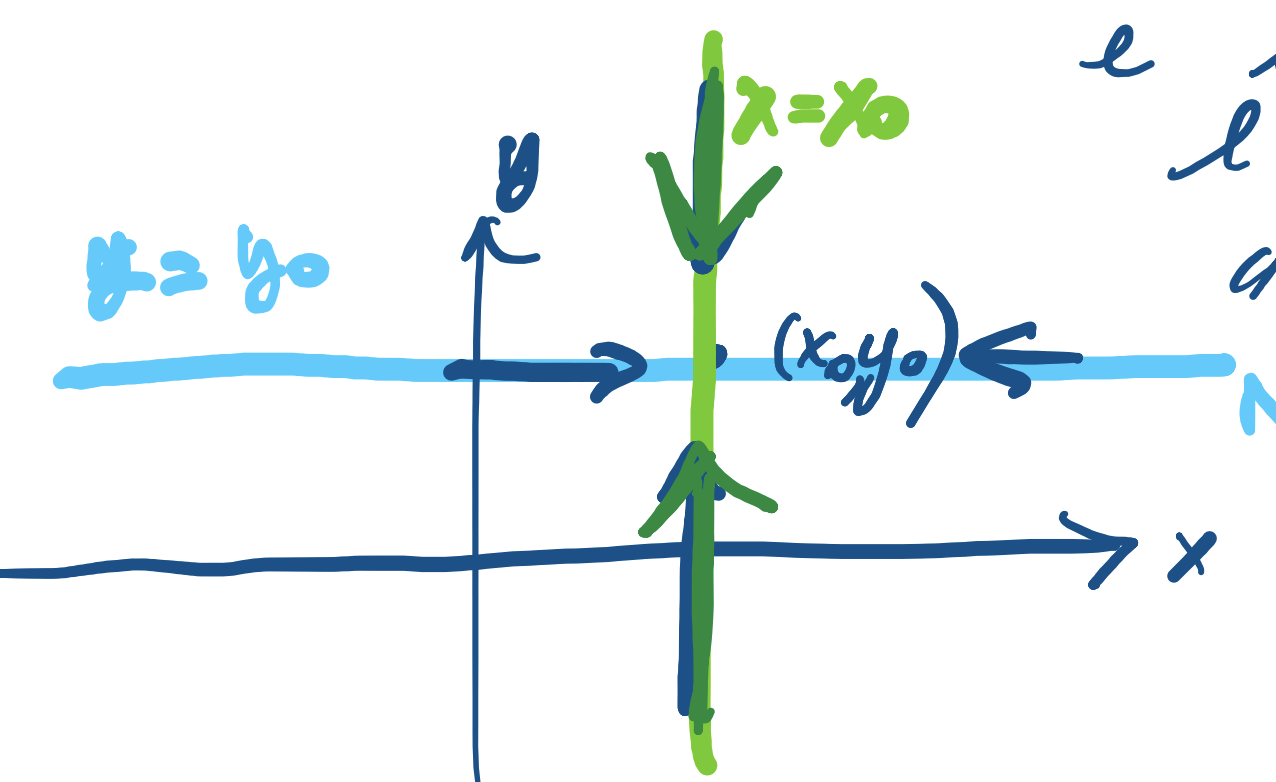
\includegraphics[width=4.2cm]{images/derivata-parziale.png}
\end{wrapfigure}

Passiamo ora a considerare una funzione $f: \mathbb{R}^2 \to \mathbb{R}$ e vediamo come estendere questi concetti ad una funzione in più variabili (in particolare in 2). Per fare questo introduciamo il primo concetto che è quello di \textbf{derivata parziale} che si bassa su tenere fissa una variabile in $\mathbb{R}^2$ e lasciamo variare l'altra.

\begin{definition}[Derivata parzialmente rispetto a x]
Data una funzione $f: \mathbb{R}^2 \to \mathbb{R}$ e $(x_0,y_0)\in \mathbb{R}^2$ si dice che $f$ è \textbf{derivabile parzialmente rispetto a x}  nel punto $(x_0,y_0)$ se $\lim\limits_{t\to 0}\frac{f(x_0 + t, y) - f(x_0,y_0)}{t}$ (rapporto incrementale su la sola variabile x) esiste ed è finito. Se tale limite esiste ed è finita si dice \textbf{derivata parziale rispetto a x} di $f$ in $(x_0,y_0)$ e si indica con uno delle seguente notazioni:
\vspace{-5pt}
\[\frac{\partial f}{\partial x}(x_0,y_0) \hspace{.5cm}o\hspace{.5cm} f_x(x_0,y_0) \hspace{.5cm}o\hspace{.5cm} D_x f(x_0,y_0)\]
\end{definition}
\hspace{-15pt}Analogamente possiamo definire la derivata parziale rispetto a y.
\begin{definition}[Derivata parzialmente rispetto a y]
Si dice che $f$ è \textbf{derivabile parzialmente rispetto a y}  nel punto $(x_0,y_0)$ se $\lim\limits_{t\to 0}\frac{f(x_0, y+t) - f(x_0,y_0)}{t}$ (rapporto incrementale su la sola variabile y) esiste ed è finito. Se tale limite esiste ed è finita si dice \textbf{derivata parziale rispetto a y} di $f$ in $(x_0,y_0)$ e si indica con uno delle seguente notazioni:
\vspace{-5pt}
\[\frac{\partial f}{\partial y}(x_0,y_0) \hspace{.5cm}o\hspace{.5cm} f_y(x_0,y_0) \hspace{.5cm}o\hspace{.5cm} D_y f(x_0,y_0)\]
\end{definition}

\begin{observation}
I limiti coinvolti nella definizione di derivata parziale sono limiti in una variabile (cioè in $\mathbb{R}$) infatti sono limiti del tipo $\lim\limits_{t\to 0}$.
\end{observation}

\hspace{-15pt}Possiamo vedere queste derivate geometricamente.
$f_x(x_0,y_0)$, consideriamo la retta parallela all'asse x e passante per il punto $(x_0,y-0)$, vuol dire che $y_0$ resta fissato e lascio variare x. In forma parametrica questa retta la posso scrivere come $(x_0,y_0) + t(1,0) = (x_o + t, y_0)$, guardo la funzione $f$ ristretta a questa retta, quindi $f(x_0 + t, y_0) = g(t)$ (mi muovo con il parametro t).\\
\begin{wrapfigure}[7]{l}{5.2cm}
    \vspace{-10pt}
    \centering
    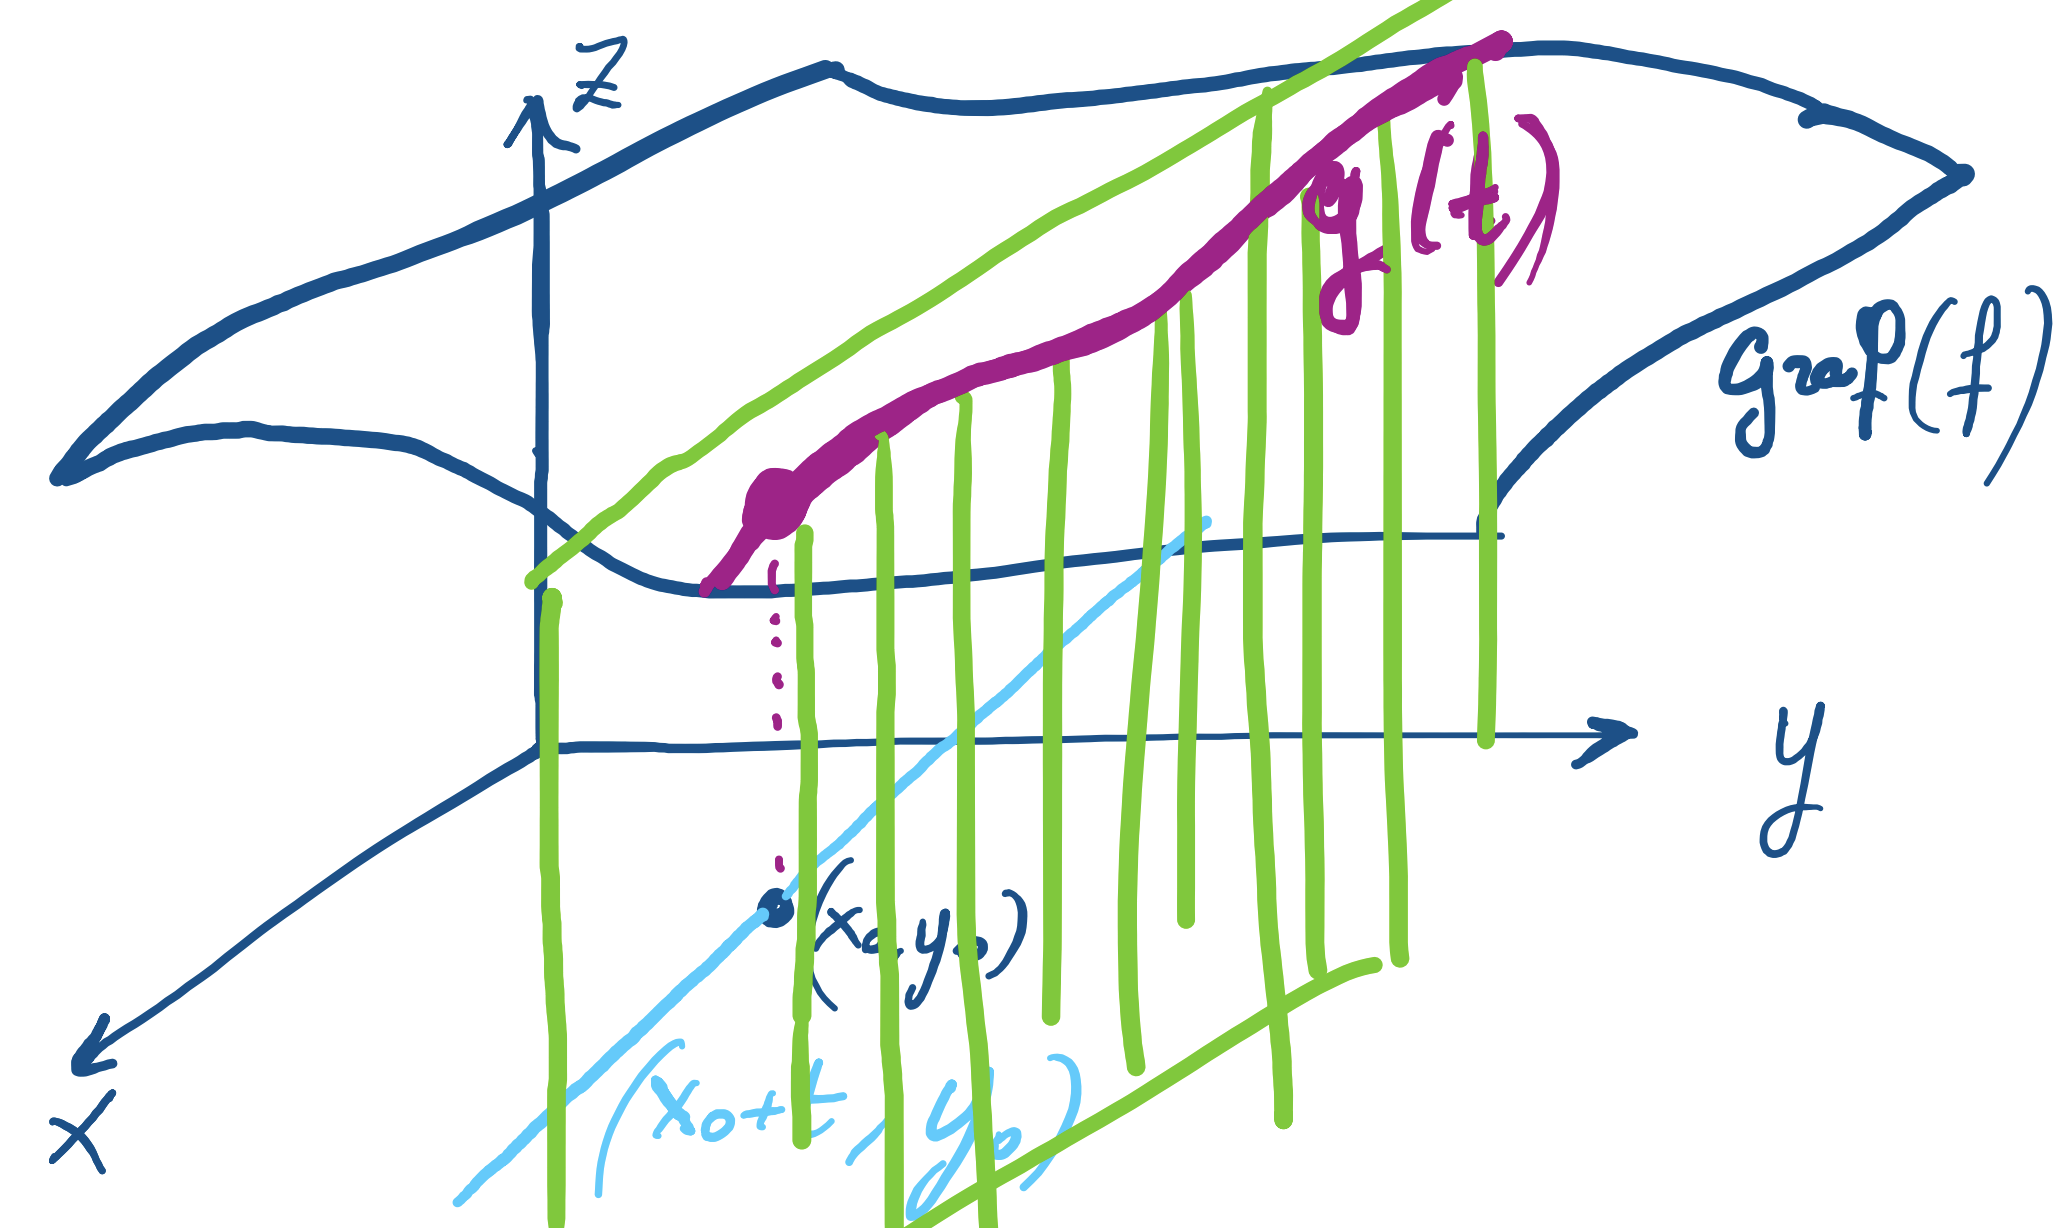
\includegraphics[width=4.7cm]{images/derivata-parziale-geometricamente.png}
\end{wrapfigure}
Geometricamente $g(t)$ lo ottengo come l'intersezione del grafico di $f(x,y)$ con il piano perpendicolare al piano $xy$e contente la retta $(x_0+t,y_0)$. La derivata di $g(t)$ in $t=0$ quindi $g'(0)$ è proprio $f_x (x_0,y_0)$ perché sarebbe $\lim\limits_{t\to 0}\frac{g(t) - g(0)}{y} = \lim\limits_{t\to 0}\frac{f(x_0+t, y_0) - f(x_0,y_0)}{y} = f_x(x_0,y_0)$.\\
Analogamente per la derivata parziale $f_t(x_0,y_0)$ dove però definirò $h(t) = f(x_0, y_0+t)$, $h'(0) = f_y(x_0,y_0)$.\\\\
Nel caso di $f: \mathbb{R}^2 \to \mathbb{R}$ ho 2 derivate parziali, ma posso estendere questa definizione anche per n variabili.

\begin{definition}
Dato $f: \mathbb{R}^2 \to \mathbb{R}$ ì, un $x_0 \in \mathbb{R}^2$ dove $x_0 = (x_{01}, x_{02}, \cdots, x_{0n})$ si dice \textbf{derivata parziale} di $f$ rispetto alla variabile $x_k$ se $\lim\limits_{t\to 0 }\frac{f(x_0 + te_k) - f(x_0)}{t}$ esiste  ed è finito. Inoltre se questo limite esiste ed è finito ì, tale limite viene indicato con $\frac{\partial f}{\partial x_k}(x_0)$. 
\end{definition}

\begin{observation}
Abbiamo $x_0 \in \mathbb{R}^2$ quindi $x_0 = (x_{01}, x_{02}, \cdots, x_{on})$ fare $f(x_0 + te_k)$ vuol dire che, avendo $\{e_1, \cdots, e_n\}$ base canonica di $\mathbb{R}^n$ abbiamo che $e_1 = (1,0, \cdots, 0)$ genera l'asse $x_1$, $e_2 = (0,1,\cdots, 0)$ genera l'asse $x_2$ $e_k = (0,\cdots, 1, 0, \cdots, 0)$ genera l'asse $x_k$ e $e_n = (0,\cdots, 0,\cdots, 1)$ genera l'asse $x_n$. Quindi fare $f(x_0 + te_k)$ aggiungo t solo sulla k-esima variabile, nel caso di $\mathbb{R}^2$ fare $f(x_0+te_1)$ corrispondeva a muoversi nella direzione x e quindi calcolare la derivata parziale rispetto a x ed analogamente $(x_0+te_1)$ corrispondeva a muoversi nella direzione y e quindi calcolare la derivata parziale rispetto a y.\\
Quando $f: \mathbb{R}^n \to \mathbb{R}$ ho n direzione e quindi n vettori della base canonica, questo indica che una funzione di n variabili ha n derivata parziali ($\frac{\partial f}{\partial x_1}, \frac{\partial f}{\partial x_2}, \cdots, \frac{\partial f}{\partial x_n}$).
\end{observation}

\subsection{Derivata direzionale}
\begin{definition}[Derivata direzionale in $\mathbb{R}^2$]
Sia $f: \mathbb{R}^2 \to \mathbb{R}$, e $(x_0,y_0) \in \mathbb{R}^2$ e sia dato $v = (\alpha, \beta) \in \mathbb{R}^2$ un vettore di $\mathbb{R}^2$ non nullo (quindi $\alpha^2 + \beta^2 \neq 0$). Allora il limite $\lim\limits_{t \to 0}\frac{f(x_0 + t\alpha, y_o + t\beta) - f(x_0,y_0)}{t}$ se esiste ed è finito si dice \textbf{derivata direzionale} di $f$ in $(x_0, y_0)$ rispetto alla direzione $v = (\alpha, \beta)$ e si indica con $\frac{\partial f}{\partial v}(x_0,y_0)$
\end{definition}

\begin{wrapfigure}[7]{l}{5.7cm}
    \vspace{-10pt}
    \centering
    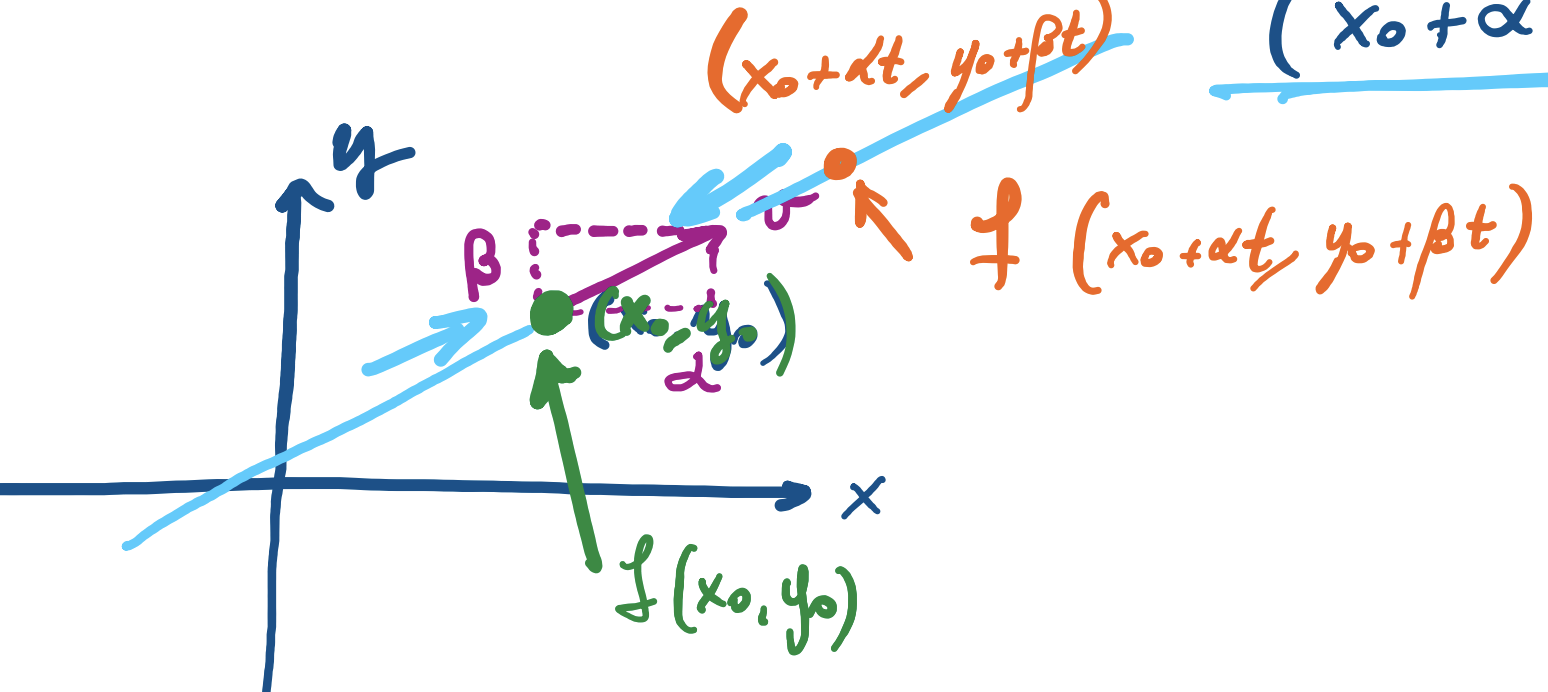
\includegraphics[width=5.5cm]{images/deri-direzionale.png}
\end{wrapfigure}

\hspace{-15pt}L'interpretazione geometrica di una derivata direzionale corrisponde a muoversi lungo la retta di equazione parametrica $(x_0, y_0) + t(\alpha, \beta) = (x_0 + \alpha t, y_0 + \beta t)$. \\
Scrivere quindi derivata direzionale rispetto alla direzione v significa restringere la funzione alla retta passante in ($x_0,y_0$) e con direzione $v$ e calcolarne la derivata rispetto a t nel punto $t=0$. \\\\
Definiamo $g(t) = f(x_0 + t\alpha, y_0 + t\beta)$ e $g'(0) = \frac{\partial f}{\partial v}(x_0, y_0)$ (derivata in una dimensione), e $g'(0) = \lim\limits_{t\to 0}\frac{g(t) - g(0)}{t} =\lim\limits_{t\to 0}\frac{f(x_0 + t\alpha + t\beta) - f(x_0,y_0)}{t}$ e questo corrisponde a $\frac{\partial f}{\partial v}(x_0,y_0)$ con $v=(\alpha, \beta)$.\\
Anche in questo caso, come per per derivate parziali, $g(t)$ è la funzione che ottengo intersecando il grafico di $f$ con il piano perpendicolare al piano xy e contente la retta passante per $(x_0,y_0)$ e con direzione v.\\\\
Analogamente possiamo definire al derivata direzione in n dimensioni.

\begin{definition}[Derivata direzionale in $\mathbb{R}^n$]
Sia $f: \mathbb{R}^2 \to \mathbb{R}$, e $x_0 \in \mathbb{R}^n$ ($x_0 = (x_{01}, x_{02}, \cdots, x_{0m})$ vettore) e sia dato $v \in \mathbb{R}^n$ con $v= (v_1, v_2, \cdots, v_n)$ e $v \neq 0$, definiamo $\frac{\partial f}{\partial v}(x_0)$, se esiste ed è finito, come $\lim\limits_{t\to 0}\frac{f(x_0 + tv) - f(x_0)}{t}$.
\end{definition}

\begin{observation}
Anche le derivate direzionali sono definite tramite limiti in una variabile (t paramento della retta di direzione v e passante per $x_0 \in \mathbb{R}^n$).
\end{observation}

\begin{definition}[Gradiente]
Data una $f: \mathbb{R}^n\to \mathbb{R}$, si dice \textbf{gradiente} di $f$ in $x_0 \in \mathbb{R}^n$ che ha come componenti le derivate parziali di $f$ in $x_0$ e si indica con $\nabla f(x_0) = (\frac{\partial f}{\partial x_1}(x_0), \frac{\partial f}{\partial x_2}(x_0), \cdots, \frac{\partial f}{\partial x_n}(x_0))$.
\end{definition}

\subsection{Differenziabilità di una funzione}
Ricordiamo che nel caso di una dimensione $f: \mathbb{R}\to \mathbb{R}$ si dice che $f$ è differenziabile se in $x_0$ esiste un numero reale $\alpha \in \mathbb{R}$ tale che $f(x_0 + h) = f(x_0) + \alpha \cdot h + o(h)$ con $h \in \mathbb{R}$ e $h\to 0$, dobbiamo definire una funzione differenziale in più variabili andando a generalizzare questa definizione.
\begin{definition}[Differenziabilità in $\mathbb{R}^2$]
Dato un $f: \mathbb{R}^2 \to \mathbb{R}$, un $(x_0,y_0) \in \mathbb{R}^2$ si dice che $f$ è \textbf{differenziabile} nel punto $(x_0,y_0)$ se esistono due numeri reali che chiamo $\alpha$ e $\beta$ tali che $f(x_0 + h, y_0 + k) = f(x_0, y_0) + \alpha \cdot h + \beta \cdot k + o(\sqrt{h^2 + k^2})$.
\end{definition}
\hspace{-15pt}Possiamo vedere $\alpha \cdot h + \beta \cdot k$ come il prodotto scalare $<(\alpha, \beta), (h,k)> \in \mathbb{R}$ dove $(h,k)$ è uno spostamento rispetto al punto ($x_0,y_0$) e $(\alpha, \beta)$ devono esiste per avere un differenziale di $f$, inoltre $\sqrt{h^2 + r^2}$ è uguale alla lunghezza di $(h,k)$ che quindi è uguale alla lunghezza dello spostamento, quindi l'errore in questa formula è determinata dall'o-piccolo, infatti quando scrivo $o(\sqrt{h^2 + k^2})$ significa che $\lim\limits_{(h,k)\to (0,0)}\frac{o(\sqrt{h^2 + k^2})}{\sqrt{h^2 + k^2}} = 0$ (limite in due variabili).\\\\
Da qui si può generalizzare in n dimensioni.

\begin{definition}[Differenziabilità in $\mathbb{R}^n$]
Dato un $f: \mathbb{R}^n \to \mathbb{R}$, un $x_0 \in \mathbb{R}^n$ si dice che $f$ è \textbf{differenziabile} nel punto $x_0$ se esistono un vettore $\alpha \in \mathbb{R}^n$ (devono esistere n numeri reali $\alpha_1, \cdots, \alpha_n$) tale che $f(x_0 + h) = f(x_0) + \alpha \bullet h + o(|h|)$ (norma del vettore h) per $h \to 0$ (limite in n variabili).
\end{definition}

\begin{theorem}\label{teorema-differenziabilità}
Supponiamo che $f: \mathbb{R}^n \to \mathbb{R}$ sia differenziabile in $x_0 \in \mathbb{R}^n$, allora valgono le seguenti proprietà:
\begin{enumerate}
    \item $f$ è continua in $x_0$.
    \item Esistono le derivate parziali di $f$ in $x_0$ e queste sono le componenti del vettore $\alpha = (\frac{\partial f}{\partial x_1}(x_0), \cdots, \frac{\partial f}{\partial x_n}(x_0)) = \nabla f(x_0)$.
    \item Esistono tutte le derivate direzioni di $f$ in $x_0$ e sono date da $\forall \: v \in \mathbb{R}^n \: \exists \: \frac{\partial f}{\partial v}(x_0)$ e $\frac{\partial f}{\partial v}(x_0) = \alpha \cdot v$ dove $\alpha = \nabla f(x_0)$, quindi vale che $\frac{\partial f}{\partial v}(x_0) = \nabla f(x_0) \cdot v$.
\end{enumerate}
\end{theorem}

\begin{note}
Notare bene che questo teorema vale per un solo verso e non viceversa, cioè può succedere che in $x_0$ esistano tutte le derivate parziali ma la funzione non è nemmeno continua in $x_0$ (quindi non differenziabile), quindi se $\exists$ derivata parziale non è detto che la funzione sia differenziabile.
\end{note}

\begin{example}
Consideriamo $f(x,y) = \begin{cases}(\frac{x^2 \cdot y}{x^4 + y^2})^2 & (x,y) \neq 0 \\ 0 & (x,y) = (0,0)\end{cases}$ Verifichiamo che nel punto $(x_0, y_0) = (0,0)$ esistono derivate direzionali e sono nulle, ma $f$ non è nemmeno continua.\\
Fisso $v = (\alpha, \beta) \in \mathbb{R}^2$, $(x_0, y_0) = (0,0)$ e poi calcolo la derivata direzionale $\lim\limits_{t \to 0}\frac{f(x_0 + t\alpha, y_0 + t\beta) - f(x_0,y_0)}{t} = \frac{1}{t}\bigg(\frac{t^2\alpha^2 \cdot t\beta}{2t^4\alpha^4 + t\beta^2}\bigg)^2 = t\bigg(\frac{\alpha^2\beta}{t^2\alpha^2 + \beta^2}\bigg)^2 = 0$ quindi $\frac{\partial f}{\partial v}(0,0) = 0$.
\end{example}

\begin{demostration}
Dimostriamo ora il punto (3) del teorema visto quindi che, se $f$ è differenziabile in $x_0 \in \mathbb{R}^n$ allora esistono tutte le derivate direzionali di $f$ in $x_0$, $\frac{\partial f}{\partial v}(x_0) = \alpha \cdot v$.\\\\
La nostra ipotesi è che $f$ è differenziabili in $x_0$, questo vuol dire che $\exists$ un vettore $\alpha \in \mathbb{R}^n$ tale che $f(x_o + h) = f(x_0) + \alpha \cdot h + o(|h|)$ per $h\to 0$. Fissiamo ora una direzione $v \in \mathbb{R}^n$ con $v\neq 0$, per definizione $\frac{\partial f}{\partial v}(c_0) = \lim\limits_{t\to 0}\frac{f(x_0 + tv) - f(x_0}{t}$, ora uso l'ipotesi di differenziabilità e posso usarla perché la formula della diff. vale quando $h\to 0$ e quindi scelgo $g = t \cdot v$ e posso fare questa scelta perché $v \in \mathbb{R}^n$  $(t\cdot v)\in \mathbb{R}^n$ perché pure $t \in \mathbb{R}^n$.\\\\
Quindi sostituiamo $h$ con $tv$ e viene $\lim\limits_{t\to 0}\frac{f(x_0) + t(\alpha \cdot v) + o(|tv|) - f(x_0)}{t} = \frac{t(\alpha\cdot v)}{t} + \frac{o(|tv|)}{t} = (\alpha \cdot v) + \lim\limits_{t\to 0}\frac{o(|tv|)}{t|v|} \cdot |v|$, la parte $|v| \neq 0$ è la norma di $v$, mentre $\frac{o(|tv|)}{t|v|}\to 0$ per definizione di o-piccolo, quindi questo limite fa $(\alpha \cdot v) + 0 = (\alpha \cdot v)$.\\
Quindi ho ottenuto che $\frac{\partial f}{\partial v}(c_0) = \alpha \cdot v$
\end{demostration}

\begin{observation}
Osserviamo che le derivate parziali sono casi particolari di derivate direzionali, corrispondo infatti alla scelta $v = e_k$ (vettori della base canonica).\\\\ Quindi la dimostrazione appena fatta ci mostra anche l'esistenza delle derivate parziali (2) del teorema e la formula $\frac{\partial f}{\partial x_k}(x_0) = \frac{\partial f}{\partial e_k}(x_0) = \alpha \cdot e_k = \alpha_k$ dove $e_k$ è il k-esimo vettore della base canonica di $\mathbb{R}^n$ (quindi è il vettore $0,\cdots,0, 1, 0 \cdots, 0$), e $\alpha_k$ sarà la k-esima componente di $\alpha$, ma $\alpha$ era il vettore nella formula di differenziabilità di $f$ con $\alpha_k = \frac{\partial f}{\alpha x_k} \Longrightarrow \alpha = \nabla f(x_0)$. \\
Quindi se $f$ è differenziabile in $x_0$, possiamo in conclusione scrivere che $f(x_0 + h) = f(x_0) + \nabla f(x_0) \cdot h + o(|h|)$ per $h\to 0$.
Inoltre le derivate direzionali sono date dalle formule $\frac{\partial f}{\partial v}(x_0) = \nabla f(x_0)\cdot v$.
\end{observation}

\begin{observation}
Le formule e le conclusioni del teorema valgono per qualsiasi direzione v. Nel definire le derivate direzionali possiamo in realtà limitarci alle direzioni v con $|v| = 1$, perché comunque in questo modo descrivo comunque tutte le possibili rette in cui mi muovo.
\end{observation}

\hspace{-15pt}Ora chiediamoci quale sia il significato geometrico del gradiente, per rispondere a questa domanda dobbiamo prima chiederci in quale direzione la derivata direzionale è massima o minima, per fare questo ci atteniamo all'algebra lineare che dice che $\frac{\partial f}{\partial v}(v_0) = \nabla f(x_0) \cdot v$ può essere scritto come $|\nabla f(x_0)| \cdot |v| \cdot \cos{\Theta}$ dove $\cos{\Theta}$ è l'angolo compreso tra $\nabla f$ e $v$. \\
Noi ci stiamo chiedendo $\max\limits_v \frac{\partial f}{\partial v}(x_0)$, in base all'osservazione $|v| = 1$ possiamo vedere che questo massimo lo realizzo quando massimizzo $\cos{\Theta}$ e questo è massimizzato quando $\cos{\Theta} = 1$ e questo accade quando $\Theta = 0$ e questa cosa può avvenire quando l'angolo compreso tra $\nabla f$ e $v$ è zero che è possibile se e solo se scelgo come direzione quella del gradiente stesso cioè quando $v$ è parallela a $\nabla f$.\\
Quindi riassumendo $\max\limits_{|v| = 1} \frac{\partial f}{\partial v}(c_0) = \frac{\partial f}{\partial (\nabla f(x_0))}(x_0)$.
\begin{itemize}
    \item Se voglio derivata direzionale massima devo scegliere $v =$ direzione del gradiente, cioè se $v$ è parallela a $\nabla f(x_0)$ allora ho max derivata direzionale in $x_0$.
    \item Per minimizzare $\frac{\partial f}{\partial v}(x_0)$ devo prendere $\cos{\Theta} = -1$ cioè $\Theta = \pi$ cioè $v$ parallela a $-\nabla f$ cioè $v$ dovrà avere direzione opposta a quella del gradiente. Riassumendo se $v$ parallela a $-\nabla f(x_0) \Longrightarrow$ minima derivata direzionale in $x_0$.
    \item Se scelto invece $\Theta = \pm \frac{\pi}{2}$ allora avrò che $\cos{\Theta} = 0$ ed allora $\frac{\partial f}{\partial v}(x_0) = 0$ cioè se $v$ è perpendicolare alla direzione $\nabla f(x_0) \Longrightarrow$ derivata direzionale è nulla.
\end{itemize}
In conclusione possiamo vedere il significato geometrico del gradiente. Il gradiente rappresenta la direzioni di massima pendenza della funzione che stiamo considerando, cioè è la direzione in cui muoversi per salire più in fretta possibile.\\\\
Nell'analisi finora quando si scriveva $f(x_0 + h) = f(x_0) + f'(x_0) \cdot h + o(h)$ per $h\to 0$, se chiamavamo $x_o + h = x \to x_0$ allora $f(x) = f(x_0) + f'(x_0)(x - x_0) + o(x - x_0)$ per $x \to x_0$ e in questo modo il termine $f(x_0) + f'(x_0)(x - x_0)$ rappresentava la retta tangente al grafico di $f$ nel punto $(x_0, f(x_0))$; ora invece, nell'analisi in più variabili (caso $f: \mathbb{R}^2 \to \mathbb{R}$) avviamo $f(x_0 + h, y_0 + k) = f(x_0. y_0) + \frac{\partial f}{\partial x}(x_0,y_0) \cdot h + \frac{\partial f}{\partial y}(x_0, y_0) \cdot k + o(\cdots)$, la parte $\frac{\partial f}{\partial x}(x_0,y_0) \cdot h + \frac{\partial f}{\partial y}(x_0, y_0)$ sarebbe come scrivere $\nabla f(x_0, y_0) \bullet (h,k)$, facendo come prima posso chiamare $x_0  + h = x \to x_0$ e $y_0 + k = y \to y_0$ e riscrivere $f(x,y) = f(x_0, y_0) + \frac{\partial f}{\partial x}(x_0,y_0)\cdot (x - x_0) + \frac{\partial f}{\partial y} (x_0, y_0) \cdot (y - y_0) + o(\cdots)$, questo per $x \to x_0$ e $y \to y_0$. In conclusione quello che otteniamo nell'analisi in più variabile $f(x_0, y_0) + \frac{\partial f}{\partial x}(x_0,y_0)\cdot (x - x_0) + \frac{\partial f}{\partial y} (x_0, y_0) \cdot (y - y_0)$ mi darà un piano tangente al grafico di $f$ nel punto $(x_0, y_0, f(x_0,y_0))$.

\subsection{Calcolo derivate parziali}
Innanzitutto vediamo come calcolare il vettore $\alpha$. Noi sappiamo che se la funzione è differenziabile e so calcolare le derivate parziali allora $\alpha = \nabla f(x_0, y_0)$. Se so fare calcolare le derivate parziali e se riesco a dimostrare che la funzione $f(x,y)$ è differenziabile allora $\alpha$ è il gradiente di $f$ nel punto $(x_0, y_0)$. (vettore che ha componenti le derivate parziali di $f$ in $x_0, y_0$).\\\\
Ora invece vediamo come calcolare le derivate direzione. Per loro bisogna come prima sapere se la funzione è differenziabile e calcolare le derivate parziali, allora le derivate direzionali nella direzione di $v$ $(v \in \mathbb{R}^2)$ sono date da $\frac{\partial f}{\partial v} = \nabla f \cdot v$.\\\\
Quindi bisogna sappiamo se la funzione è differenziabile e calcolare le derivate parziali sappiamo che $\frac{\partial f}{\partial v} = \nabla f \cdot v$ e che $\alpha = \nabla f(x_0, y_0)$.\\
Attenzione questo vale solo se $f$ è differenziabile perché se $f$ non è differenziabile può succedere che esistano comunque le derivate direzionali ma non saranno date dalla formula $\frac{\partial f}{\partial v} = \nabla f \cdot v$.\\\\
Campiamo ora come calcolare le derivate parziali. Per il calcolo delle derivate parziali usiamo le stesse regole dell'analisi vista fin'ora (1 dimensione), e questo lo facciamo derivando solo rispetto alla variabile che ci interessa, cioè andiamo a trattare le altre variabili come fossero costanti. Data una funzione $f: \mathbb{R}^n \to \mathbb{R}$, $\frac{\partial f}{\partial x_k}$, $f(x_1, \cdots, x_k, \cdots, x_n)$ farò $f(x_k, \cdots \: costanti)$.

\begin{example}
Consideriamo una funzione $f: \mathbb{R}^2 \to \mathbb{R}$ definita come $f(x,y) = x^2 + y^3$ (in questo caso vedo $y^3$ come costante e derivo $x^2$). Per calcolare $\frac{\partial f}{\partial x}(x,y) = f_x(x,y) = 2x$ infatti se dico che $g(x) = x^2$, $f(x,y) = g(x) + y^2$, $f_x(x,y) = g'(x) + 0$. \\
Se invece voglio calcolare $\frac{\partial f}{\partial y}(x,y) = f_y(x,y) = (x \: costante) = 3y^2$.
\end{example}

\begin{example}
Facciamo altri esempi di derivate parziali.
\begin{itemize}
    \item Prendiamo $f(x,y) = x^2 \cdot y^3$. Se faccio $f_x(x,y) = y^3 \cdot (2x) = 2x\cdot y^3$. Mentre $f_y(x,y) = x^2 \cdot 3y^2$.
    \item $f(x,y) = \sin(xy^2)$, $f (x,y) = \sin(x \cdot c)$ dove $c = y^2$ quindi rispetto a $x$ ho $f_x(x,y) = \cos{xy^2} \cdot y^2$ mentre rispetto a y ho $f_y (x,y) = \cos(xy^2)x \cdot 2y$.
    \item Facciamo un esempio in $\mathbb{R}^3$ quindi $f: \mathbb{R}^3 \to \mathbb{R}$ e con $f(x,y,z) = x \cdot e^{yz^2}$. In questo caso ci saranno allora 3 derivate parziali.\\
    $f_x(x,y,z) = e^{yz^2}$ (teniamo $y,z$ costanti), $f_y(x,y,z) = x \cdot e^{yz^2} \cdot z^2$ (teniamo $x,z$ costanti), $f_z(x,y,z) = x \cdot e^{yz^2} \cdot 2zy$ (teniamo $y,x$ costanti).
    \item $f(x,y) = e^{xy} \cdot \cos{y}$, $f_x(x,y) = ye^{xy}\cdot \cos{y}$, se invece vado a fare $f_y (x,y) = x\cos{y}e^{xy} - \sin{y} e^{xy}$.
    \item $f(x,y) = \log(1 + x^2 + y^4)$ con $f:\mathbb{R}^2 \to \mathbb{R}$ calcoliamo $f_x(x,y) = \frac{2x + y^4}{1 + x^2 + y^4}$, $f_y(x,y) = \frac{4y^3}{1 + x^2 +y^4}$.
    \item $f(x,y) = x^y$, $f_x(x,y) = yx^{y-1}$ mentre $f(x,y) = a^y = e^{\log(a)^y} = e^{y\log(a)} = e^{y \log(a)} \cdot \log(a) = a^y \cdot \log(a)$ e quindi $f_y(x,y) = x^y \cdot \log(x)$
\end{itemize}
\end{example}

\subsection{Interpretazione geometrica gradiente}
Ora vogliamo specificare la relazione fra il gradiente e gli insiemi di livello. Abbiamo detto che il gradiente ci da la direzione in cui la funzione varia più velocemente mentre gli insiemi di livello ci dice l'insieme dove la funzione ha lo stesso valore, detto questo prendiamo $f:\mathbb{R}^2 \to \mathbb{R}$, consideriamo $f(x,y) = x^2 + y^2$, gli insiemi di livello definiti da $\{(x,y) \in \mathbb{R}^2 \::\: f(x,y) = \lambda\}$, che sono circonferenze concentriche con centro dell'origini e raggio $\lambda$.\\

\begin{wrapfigure}[7]{r}{5.7cm}
    \vspace{-30pt}
    \centering
    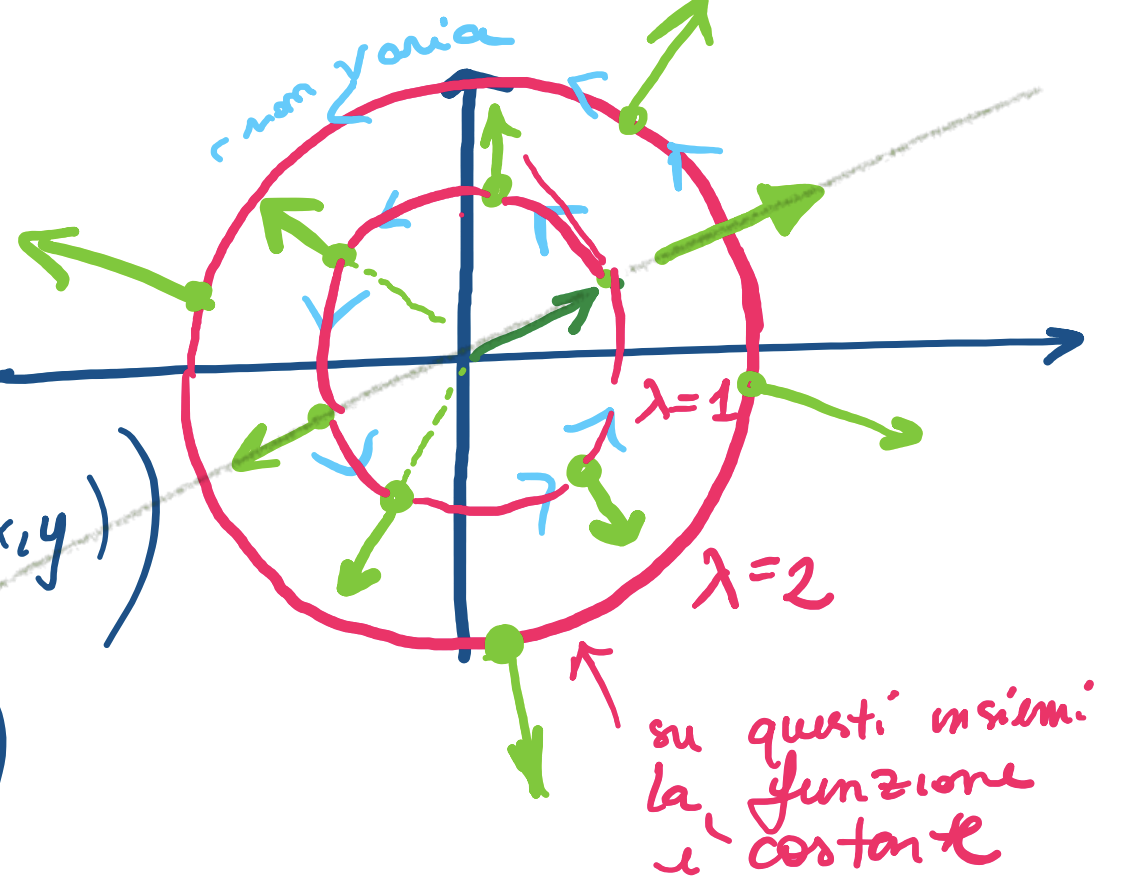
\includegraphics[width=5cm]{images/sign-geom-gradiante.png}
\end{wrapfigure}

Calcoliamo $\nabla f(x,y) = \big( \frac{\partial f}{\partial x}(x,y), \frac{\partial f}{\partial y}(x,y) = (2x, 2y)$, $\nabla f(x,y) = 2 \cdot (x,y)$, se prendo un qualsiasi punto $(x,y) \in \mathbb{R}$ dico che in quel punto il vettore gradiente è 2 volte il vettore stesso. In generale, geometricamente il gradiente si rappresenta come "campo di vettori": in ogni punto del dominio disegno un vettore (il gradiente) che mi sta indicando la direzione per salire con la massima pendenza.

\begin{observation}
Il gradiente è sempre perpendicolare agli insiemi di livello e punta verso i $\lambda$ crescenti.
\end{observation}

\begin{example}
Consideriamo $f:\mathbb{R}^2 \to \mathbb{R}$, $f(x,y) = x^2 -xy$ calcolare $\frac{\partial f}{\partial v}$ nel punto $(x_0,y_0) = (-1,2)$ con $v = (1,3)$.
\end{example}
\begin{wrapfigure}[6]{l}{5cm}
    \vspace{-10pt}
    \centering
    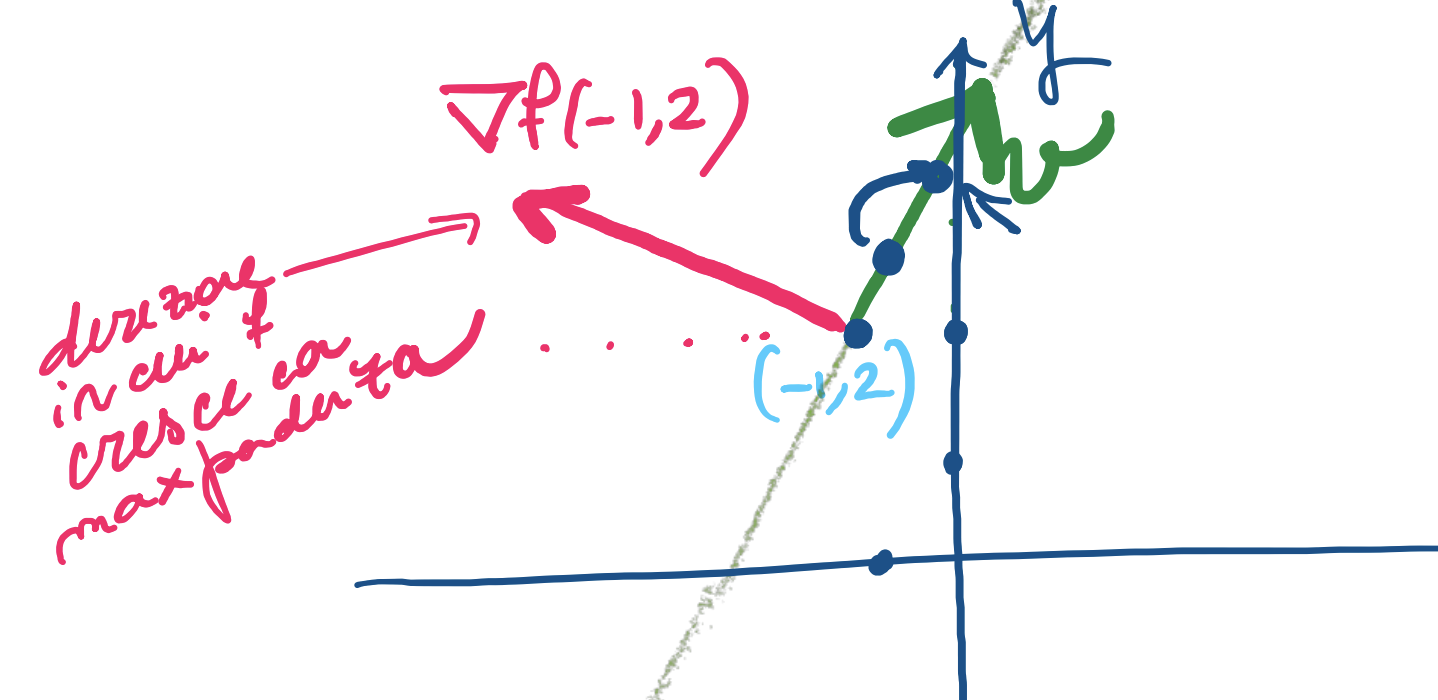
\includegraphics[width=4.7cm]{images/ess-gradiante-1.png}
\end{wrapfigure}
Noi sappiamo che se so calcolare $\nabla f \Longrightarrow \frac{\partial f}{\partial v} = \nabla f(x_0, y_0) \cdot v = (\frac{\partial f}{\partial x}, \frac{\partial f}{\partial y}) = (2x - y, -x)$ sostituiamo con $(x_0,y_0)$ ed otteniamo $\nabla f(x_0,y_0) = \nabla f(-1,2) = (-4, 1)$.\\
Sappiamo che $\frac{\partial f}{\partial v}(-1,2) = \nabla f(-1,2) \cdot v = (-4,1)\cdot(1,3) = -4 + 3 = -1 < 0$ e quindi $f$ sta scendendo.\\
Geometricamente immaginiamoci un omino che si trova sul grafico di $f$ nel punto corrispondente a $(-1,2)$ (il punto sul grafico (-2,2,$f(-1,2)$) = (-1,2,3)) e si muove nella direzione $(1,3)$ si trova a scendere.

\begin{example}
Prendiamo $f(x,y) = xy$.
\end{example}
\begin{wrapfigure}[8]{l}{5cm}
    \vspace{-10pt}
    \centering
    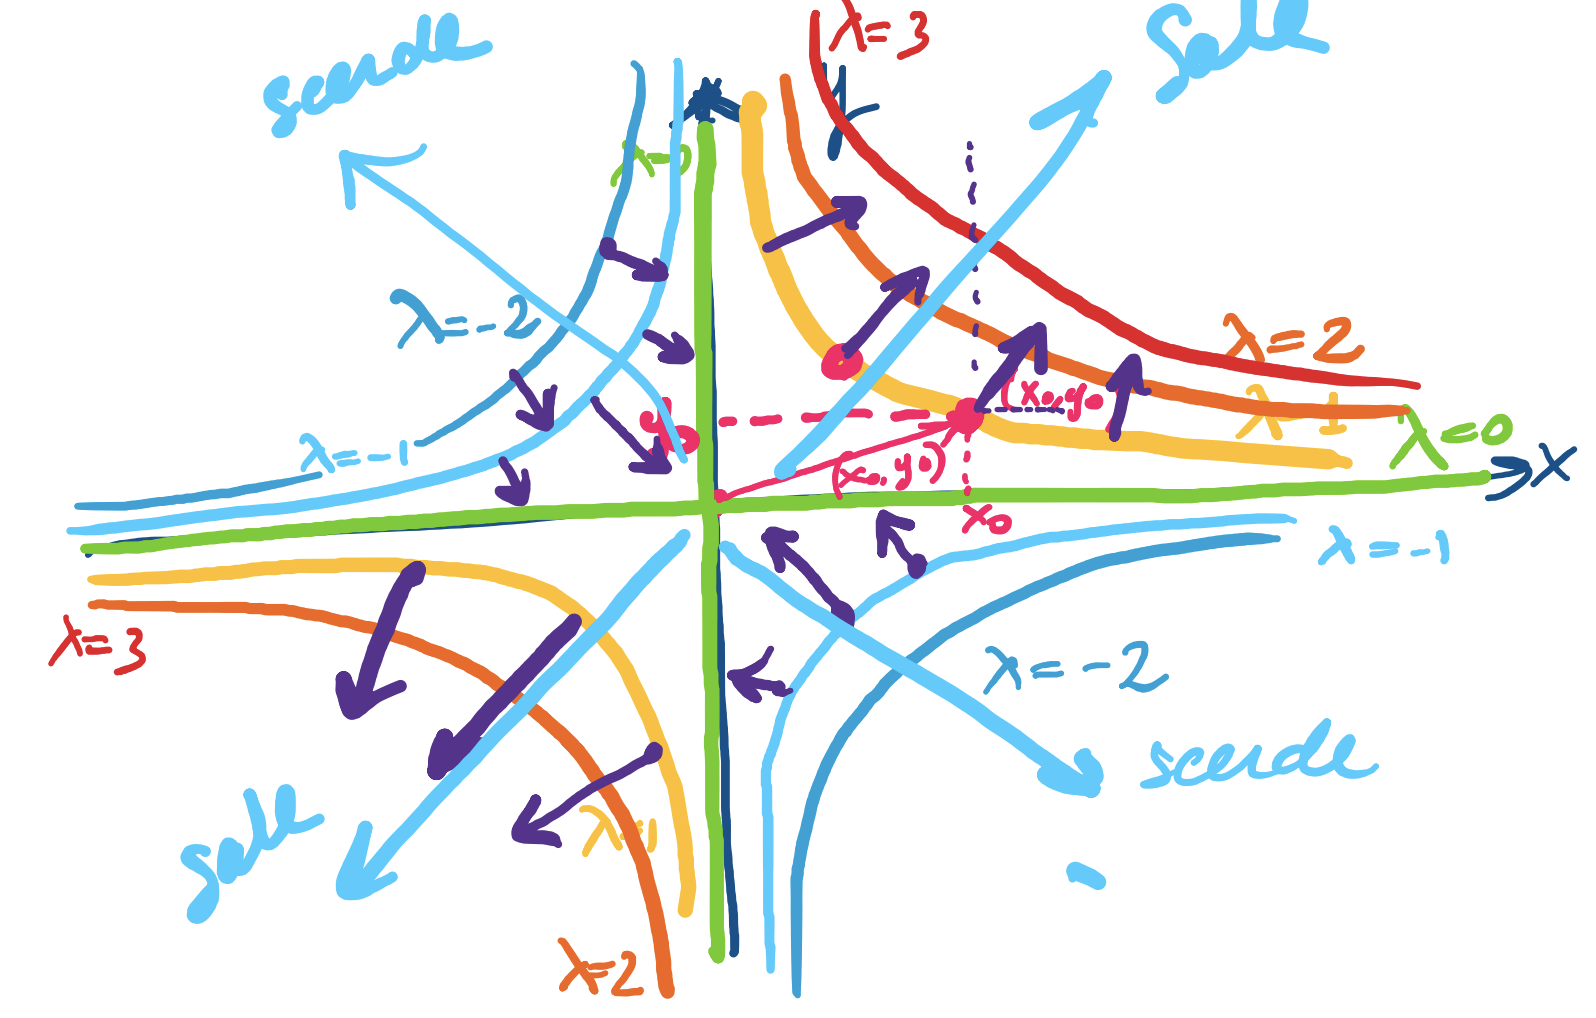
\includegraphics[width=4.8cm]{images/ess-gradiane-2.png}
\end{wrapfigure}
Disegniamo il gradiente della funzione (che vuol dire mettersi nello spazio di partenza e per ogni punto di questo spazio disegnare un vettore che indica la direzione del gradiente, nel nostro caso ovviamente lo si fa solo per alcuni punti). \\
Iniziamo a vedere $\nabla f(x,y) = (y,x)$ (calcolo la derivata parziale per x e y). Le linee di livello sono definite come $\{(x,y)\in \mathbb{R}^2 \::\: xy = \lambda\}$. In un punto $(x_0,y_0)$ il gradiente avrà come ascissa $y_0$ e come originata $x_0$ e questo per ogni punto. 


\subsection{Teorema del differenziale totale}
Quello che ci stiamo chiedendo è come posso dimostrare che $f(x,y)$ è differenziabile in $x_0,y_0$. Per farlo si può agire in due modi, o usare la definizione, ma sconsigliato perché molto complesso, oppure utilizzare il seguente teorema.

\begin{theorem}[Teorema del differenziale totale]
Se le derivate parziali di $f$ esistono e sono continue allora $f$ è differenziabile in quel punto.
\end{theorem}
\hspace{-15pt}A livello pratico, se non si incontrano problemi nel calcolare le derivate parziali, la funzione è differenziabile.\\\\
Quindi per le domande che si eravamo posti all'inizio: come calcolare il vettore $\alpha$ e come calcolare le derivate direzione possiamo avere una risposta visto che dovevamo dove sapere se la funzione è differenziabile e calcolare le derivate parziali, ed ora possiamo per il primo punto fare come scritto nel paragrafo precedente, e per il secondo punto usare questo teorema.

